\section*{Abstract}

When oil and gas wellbores are drilled, barriers must be put in place to ensure that fluids do not leak out of the wellbore.
%Wellbore leakage can lead to environmental damage, loss of pressure at the wellhead, and consequently, loss of production.
An important yet vulnerable barrier is the cement annulus and is created through a process known as primary cementing.
Every well has unique subsurface conditions, and so no cement slurry mix design both performs well and is economical for all wells.
%Although some general guidelines and analytical techniques exist for approximating the performance of a cement slurry mix, the mechanics of primary cementing are complex.
Computational methods can help better understand primary cementing and aid designers in determining the optimal mix.
The lattice Boltzmann method (LBM) is a promising technique for simulating primary cementing because it is well-suited for efficiently simulating non-Newtonian flow, multiphase multicomponent flow, and flow through complex geometries--namely, some of the complexities associated with the mechanics of primary cementing.
In \Fref{sec:numerical-methods}, an algorithm for simulating non-Newtonian free-surface flow using LBM is presented.
The algorithm was implemented and used to study primary cementing of a dry annulus, i.e. an annulus that is not filled with drilling mud.
More specifically, the study involved parameterizing different cement slurry flows and investigating how well each slurry flow filled different wellbore geometries.
The study is followed by conclusions and a discussion of future work.

\section{Introduction}

% what is primary cementing?

Of critical importance to drilling operations of all kinds is that barriers are placed to prevent gasses and fluids from migrating from one geological zone to another (i.e., zonal isolation is achieved)~\cite{economides19901,jackson1993effect,goodwin1992cement,dusseault2014towards,li2016theory}.
If zonal isolation is not achieved, gasses and fluids may migrate through the well to the surface and up into the atmosphere--potentially causing pollution, or at the very least, contributing to an increase in greenhouse gasses--or, worse yet, formation gasses and fluids can migrate into aquifers, potentially harming wild life and people.
Furthermore, it can be argued that the most important, yet vulnerable, barrier in terms of achieving zonal isolation of a wellbore is the cement annulus that is created between the casing and the formation.
There are various mechanisms by which this cement annulus can fail.
According to previous studies~\cite{Bit02,Che85,Lev79,Ste88,Tal93,Zul12,li2016theory}, the most prevalent failure mechanisms of the cement annulus are:
\begin{itemize}
\item Stresses developing in the cement annulus as a result of temperature gradients, moisture gradients, overburden pressure, and chemical shrinkage of the cement matrix.
These stresses can cause cracking in the cement, or debonding at either the casing--cement or cement--formation interfaces.
\item Poor fill of the annulus.
If cement slurry does not fill the annulus and if drilling mud is left behind the mud can dry, crack, and provide a weak path for fluids and gasses under pressure to push through, or if a dry hole is cemented and not filled properly, fluids and gasses can travel through channels and voids left in the annular space.
\item Gas channeling through the annulus during cement curing.
Initially, after the annulus is poured, the cement column transmits its full hydrostatic pressure against the rock formation.
As the cement annulus hydrates, it solidifies, becoming stiffer and more self-supporting.
When the column begins to support itself, the hydrostatic pressure of the cement column--against the rock formation--begins to drop.
If the hydrostatic pressure of the cement column drops below the pressure of a formation gas before the cement annulus has developed adequate strength to resist it, the formation gas can penetrate into the cement annulus and form channels, or degrade the cement annulus in other ways.
\end{itemize}
% what research has been done that is considered classical?

% why do we need modelling?
% Before the end of this paragraph--modeling is important because...

In order to better understand, and thus improve primary cementing for zonal isolation, several works have attempted to model certain aspects of the multiphase and multiphysics processes of wellbore cement placement.
For example,~\citet{Bei77} developed a mathematical model to describe the displacement of drilling mud by the the cement slurry during primary cementing.
Among their assumptions were that the flow as laminar, the process could be modeled in a quasi-steady manner, the volumetric flow rate was constant at each cross section of the flow, and the pressure fields were only dependent on the distance from the center of the annulus to either the rock formation or steel casing surface.
The model was then used to explore the effect of various parameters on the displacement efficiency of the spacer, such as the density ratio between the mud and the spacer, the viscosity ratio between the mud and the spacer, the displacement rate, the displaced phase yield stress, and the displacing phase yield stress.
It was concluded that displacement efficiency could be improved by increasing the density of the displacing phase, increasing the viscosity of the displacing phase, (in general) decreasing the displacement rate, decreasing the yield stress of the displaced phase, and increasing the yield stress of the displacing phase.
\citet{Bit02} developed a mathematical model for primary cementing of an oil well using a Hele-Shaw displacement model.
The model was more general than the model developed by~\citet{Bei77} as it used less restrictive assumptions and was able to consider an eccentric annulus.
The bulk fluid motion of the spacer and drilling mud during primary cementing were investigated.
The intended use of the model was not to make general statements about what properties of the spacer and drilling mud were desirable, but to instead be used iteratively during the design process for the cement job.
Results showed that the model was able to simulate an unyielded channel of mud left on the narrow side of the annulus.
\citet{Zul12} used a computational fluids dynamics (CFD) solver with volume of fluid (VOF) method to simulate the cementing process of a 50 ft. section of wellbore.
The model included the interfacial dynamics of, not just the spacer and drilling mud, but also the cement slurry--which was not considered in either~\citet{Bei77} or~\citet{Bit02}.
The drilling mud and cement slurry properties were kept constant, while the spacer density, viscosity, and displacement rates were varied.
\citet{Zul12} concluded that the high displacement efficiency occurred when the spacer was the same density as the drilling mud and had a smaller viscosity, similar to that of water.
The displacement efficiency was poor for all scenarios in which the spacer and cement slurry densities were equal.
\citet{zhao2016lattice} developed a model simulating primary cementing using the Lattice Boltzmann Method.
\citet{zhao2016lattice} used the model to investigate the shape of the interface between the displacing phase (i.e. cement slurry) and displaced phase (i.e. drilling mud) in a horizontal, eccentric annulus.
It was found, in general, that a greater density ratio between the displacing phase and displaced phase and lower eccentricity results in better displacement in a horizontal, eccentric annulus.

% talk about new LBM study

Overall, past studies have tended to idealize the rock formation as a straight wall.
Although this is a desirable simplification to make for capturing bulk fluid phenomena, it does not accurately describe what is happening locally at the surface of the rock formation.
Flow near the surface of the formation, and in and around the imperfections of the formation geometry, could influence the bond of the cement annulus to the rock formation, and the fill of the cement slurry very near to the rock formation.
If an adequate bond does not develop, debonding can occur as a result of thermal and mechanical stresses.
Even if most of the annulus is filled by the cement slurry, a small gap at the cement--formation interface that stretches for a long enough span of the wellbore would still be susceptible to fluid and gas migration, i.e. loss of zonal isolation.
One could even argue that the characteristic of the cement slurry flow is most important local to the cement--formation interface, and that considering imperfections in the rock formation is imperative to determining whether zonal isolation has been achieved.

The purpose of the current work is to develop a computational approach to investigate the flow of cement slurry in and around the--possibly--imperfect features of a rock formation in a vertical section of a wellbore, with the hope of better understanding what parameters of the primary cement job will lead to a good fill of the cement annulus and high bond strength at imperfect rock formation features.
The Lattice Boltzmann Method (LBM) was chosen as the most suitable modeling technique for the desired purpose because of its ability to model flow through and around complex geometries~\cite{thorne2006lattice}, such as those found at the surface of the rock formation.
LBM also has other advantages as an approach for simulating primary cementing:
\begin{itemize}
\item LBM is well-suited for simulating non-Newtonian fluids because the strain-rate tensor is computed local to each node and is second-order accurate~\cite{kruger2009shear,kruger2010second}.
Many fluids present in primary cementing such as the spacer, drilling mud, and most importantly, the cement slurry, are best modeled as non-Newtonian fluids.
\item LBM is well-suited for simulating multiphase multicomponent flow and free-surface flow because it can handle complicated interface shapes between fluid phases and components.
\item LBM is easily written in parallel.
As hardware architectures shift from one or a few cores to several CPUs, it becomes increasingly important that code for simulating complex and computationally expensive phenomena be written in parallel.
\end{itemize}
The current work focuses on the problem of cementing a dry hole, i.e. an annulus that is not filled with drilling mud prior to cementing.
In order to numerically investigate this problem, an LBM model for non-Newtonian and free-surface flow is developed.
The details of the LBM model are outlined in \Fref{sec:numerical-methods}.
What follows in \Fref{sec:results} is a preliminary study on how different characteristics of flow, e.g. cement slurry yield stress, cement slurry inlet velocity, etc., perform in regards to fill of the annulus for different wellbores with imperfect rock formation geometries.
\Fref{sec:conclusion} outlines conclusions resulting from the numerical study and a discussion of future work.

\section{Numerical Methods} \label{sec:numerical-methods}

\subsection{Lattice Boltzmann Method}

% We need to explain/justify why 2D vs. 3D

For the sake of computational efficiency, the numerical study considered a two-dimensional section of the wellbore and was simulated using the D2Q9 lattice.
Idealizing the annulus as two-dimensional limits the modeling approach in that annulus eccentricity and other three-dimensional phenomena could not be considered.
A two-dimensional representation of the annulus was deemed sufficient as the focus of this study is to establish the Lattice Boltzmann Method as a suitable method for simulating primary cementing in an annulus with an imperfect rock formation surface.
In addition to using a D2Q9 lattice, the BGK collision operator used was in the current chapter.
For more details on the fundamentals of the Lattice Boltzmann Method, the D2Q9 lattice, or the BGK collision operator, see \Fref{sec:LBM}.

\subsection{Cement Slurry Constitutive Relationship}

Cement slurry is typically modeled using a non-Newtonian constitutive relationship.
%A simple, yet accurate constitutive relationship for cement slurry is the Bingham plastic constitutive relationship.
As is commonly utilized for modeling cement and concrete fluid dynamics~\cite{ferraris2001fresh,ferraris1998testing,tattersall2003workability,roussel2007computational,roussel2015numerical,svec2012free}, the Bingham plastic constitutive relationship was utilized herein.
Bingham plastics are characterized by a plastic viscosity, which is analogous to the dynamic viscosity for Newtonian fluids, and a yield stress, which is a stress threshold that, if the shear stress does not exceed, the strain-rate is zero.
The Bingham plastic constitutive model is difficult to work with numerically.
Therefore, a smooth approximation, specifically the Papastasiou approximation, is often used~\cite{papanastasiou1987flows,chen2014simulations,tang2011bingham,Cha11,wang2008lattice,phillips2011lattice} and is used herein.
Throughout this chapter, the Papastasiou approximation with a stress growth exponent of $m = 10^6$ is used.
The BGK collision operator with $m = 10^6$ can be seen as a compromise between computational efficiency and accuracy for simulating Bingham plastic flow.
For more detail on Bingham plastics or the Papastasiou approximation, see \Fref{sec:bp}.

\subsection{Free Surface Flow}

A free-surface flow is a flow in which two-fluids exist but the dynamics of one fluid does not need to be explicitly modeled.
Typically, the phase of the primary fluid, or the fluid of interest, is a liquid; and the secondary phase that does not need to be explicitly modeled is a gas, often times air at atmospheric pressure.
The primary fluid is modeled using a standard CFD method, such as LBM, and the interaction of the secondary fluid on the primary fluid is modeled as a boundary condition at the interface between the two fluids.
The interface is what is referred to as the free-surface. \pagebreak
The advantage of modeling a multiphase multicomponent flow as a free-surface is that, because the dynamics of the secondary fluid are not explicitly tracked and simulated, the resulting algorithm is more computationally efficient in terms of both memory and CPU overhead.
The algorithm for extending the Lattice Boltzmann Method for free-surface flow used in this work follows the algorithm developed and presented in~\citet{korner2005lattice} and \citet{thurey2005interactive}.

\subsection{Capturing the Free-Surface}

Consider at each node a cell of size $\text{d}x \times \text{d}x$, where $\text{d}x$ is the distance between nodes, and the cell is centered at the node.
In order to track where the primary fluid is and where it is not (i.e. which cells contain the primary fluid), a variable is introduced, $\epsilon$, which describes what fraction of the cell is covered by the primary fluid.
Cells that have a fluid fraction of $\epsilon = 0$ contain no primary fluid (i.e. are empty); cells that have a fluid fraction of $\epsilon = 1$ are filled; and cells that have a fluid fraction $0 < \epsilon < 1$ are neither completely filled nor are they completely empty.
The fluid fraction concept is similar to how fluids are tracked in Volume of Fluid (VOF) methods~\cite{nichols1981volume}.

\subsubsection{Mass Transfer}

It is important to note that the particle distributions, $f_0, ..., f_8$, cannot be used to directly determine the fluid fraction of a cell.
Neither can the zeroth velocity moment of the particle distributions, $\rho = \sum_i f_i$.
For the algorithm used in this work, $\epsilon(\pos, t) \neq \epsilon(\mathbf{f(\pos, t)}, \rho(\pos, t))$.
Instead, each $f_i$ is related to the amount of primary fluid advection in each of the discrete velocity directions, $\pvel_i$.
To track the fluid fraction and how it changes, another variable is introduced, $M(\pos, t)$, which denotes the (primary) fluid mass in each cell.
The fluid mass is related to the fluid fraction by $\epsilon = M / \rho$.
The change in mass, $\Delta M(\pos, t)$ is related to $\mathbf{f}(\pos, t)$ and particle distribution in the neighborhood of $\pos$.
Given initial conditions on $M(\pos, 0)$ and a fixed time step size $\Delta t $, the fluid mass is determined by $M(\pos, t_n) = M(\pos, 0) + \Delta t \sum_{k=1}^n \Delta M(\pos, t_k)$.
What remains to track the fluid mass is to develop an expression for $\Delta M(\pos, t)$.

\subsubsection{Cell States} \label{sec:mass-transfer}

Each of the cells in the domain are assigned one of three states: fluid, interface, or gas.
The set of fluid, interface, and gas cells are denoted by $\fset$, $\iset$, and $\gset$, respectively.
A fluid cell is a cell that is entirely covered by the primary fluid; and a gas cell is a cell that is completely empty, or does not contain any primary fluid.
An interface is partially covered, and there is always a layer of interface cells between fluid and gas cells so that a fluid cell and a gas cell are never neighbors.
The change in mass is calculated for fluid and interface cells (i.e. $\pos \in \fset \cup \iset$) for each discrete velocity direction as follows:
\begin{equation} \label{eq:dM}
\Delta M_i(\pos, t) = \begin{cases}
f_\opidx(\pos + \pvel_i \Delta t, t) - f_i(\pos, t), & \pos \in \fset \text{ or } \pos + \pvel_i \Delta t \in \fset \\
%\left[(\epsilon(\pos, t) + \epsilon(\pos + \pvel_i \Delta t, t)) / 2\right]\left(f_\opidx(\pos + \pvel_i, t) - f_i(\pos, t)\right), & \pos \in \iset \text{ and } \pos + \pvel_i \Delta t \in \iset \\
  \frac{\epsilon(\pos, t) + \epsilon(\pos + \pvel_i \Delta t, t)}{2} (f_\opidx(\pos + \pvel_i \Delta t, t) - f_i(\pos, t)), & \pos \in \iset \text{ and } \pos + \pvel_i \Delta t \in \iset \\
0, & \pos + \pvel_i \Delta t \in \gset
\end{cases}
\end{equation}
\noindent where $\pvel_\opidx$ represents the discrete velocity vector that is opposite in direction to $\pvel_i$ (i.e. $\pvel_\opidx = - \pvel_i$).
\eqref{eq:dM} states that when the border of the two cells is covered with fluid, the change in mass for a discrete velocity direction is equal to the difference of the particle distribution entering the cell from the opposite direction and particle distribution leaving the cell in that direction.
When the border of the two cells are not covered with fluid (i.e. when both cells are interface cells) the difference is weighted by the average fluid fraction of the two cells because mass is only able to transfer across the fraction of the cell border that is covered in fluid.
The total change in mass for a cell is simply $\Delta M(\pos, t) = \sum_i \Delta M_i(\pos, t)$.
Finally, note that $\Delta M_i(\pos, t) = -\Delta M_\opidx(\pos + \pvel_i \Delta t, t)$ for all $\pos \in \domain$ where $\domain$ is the domain.
As a consequence, it is clear that $\sum_{\pos \in \domain}\Delta M(\pos, t) = 0$ (i.e. that mass is conserved for the mass transfer step).

Tracking the transport of mass throughout the domain is an important step in determining what parts of the domain contain the primary fluid and what do not.
However, for the free-surface to change shape and propagate, cells need to be able to transition state.
Cell states change based on the rule set presented in \Fref{tab:cell-transition-rules} where $\tconst$ is a small, computational constant that keeps cells from transitioning back and forth between fluid and interface, or interface and gas states in subsequent time steps.
To summarize \Fref{tab:cell-transition-rules}, gas cells cannot transition to fluid cells and vice versa, interface cells transition to fluid cells when their mass has exceeded $\rho$ by a computational constant, and gas cells when their mass is less than zero minus a computational constant.
In addition, fluid cells and gas cells transition to the interface state in order to maintain continuity of the interface, i.e. to ensure there is always a layer of interface cells in between fluid cells and gas cells.
An example of a cell transitioning state is depicted in \Fref{fig:cell-transition}.

\begin{table}
\caption{Cell state transition rules.}
\begin{tabulary}{\linewidth}{l|L|L}
\textbf{Current State} & \textbf{Condition} & \textbf{Transition} \\
\hline & \\
$(\pos, t) \in \iset$ & $M(\pos, t) < -\tconst$ & $(\pos, t + \Delta t) \rightarrow \gset$, $M(\pos, t + \Delta t) = 0$ \\
                      & $M(\pos, t) > \tconst + \rho(\pos, t)$ & $(\pos, t + \Delta t) \rightarrow \fset$, $M(\pos, t + \Delta t) = \rho(\pos, t + \Delta t)$ \\
                      & &\\
$(\pos, t) \in \fset$ & $(\pos + \pvel_i \Delta t, t + \Delta t) \in \gset$ for any $i = 1, 2, ..., 8$ & $(\pos, t + \Delta t) \rightarrow \iset$ \\
& & \\
$(\pos, t) \in \gset$ & $(\pos + \pvel_i \Delta t, t + \Delta t) \in \fset$ for any $i = 1, 2, ..., 8$ & $(\pos, t + \Delta t) \rightarrow \iset$ \\
\end{tabulary}
\label{tab:cell-transition-rules}
\end{table}

\begin{figure}
\centering
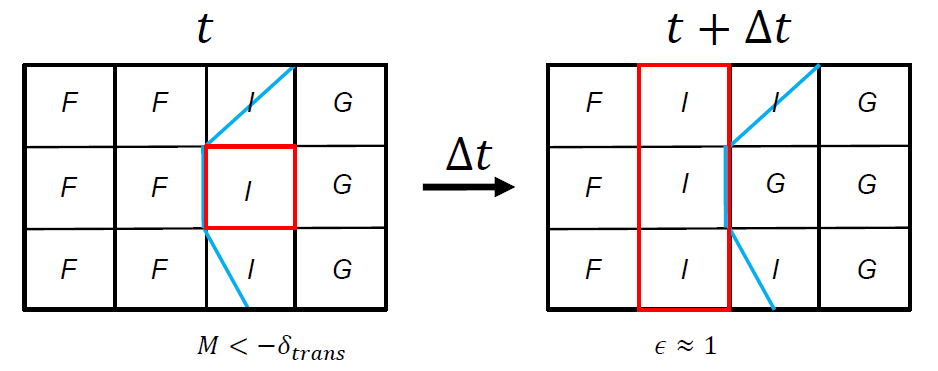
\includegraphics[width=\linewidth]{figs/cell-transition}
\caption{Example of cell state transitions.
The interface cell highlighted in red on the left is transitioned to a gas cell as it has emptied.
On the right, the three cells highlighted in red were transitioned from fluid to interface cells in order to keep the interface continuous.}
\label{fig:cell-transition}
\end{figure}

\subsubsection{Updating Cell States and Mass Redistribution} \label{sec:cell-updates}

The rules for updating cell states in \Fref{tab:cell-transition-rules} are fairly intuitive, however, there are some details that must be considered in order to ensure mass is properly conserved and interface continuity is achieved (e.g. note that if the rules outlined in \Fref{tab:cell-transition-rules} are followed naively that mass is not conserved when interface cells transition to fluid cells or gas cells).
The algorithm for updating cell states follows that which was presented in~\citet{thurey2005interactive}.
It is presented here as \Fref{algo:update-cell-states} for the sake of completeness and for outlining minor modifications.

\begin{algorithm} \small
\caption{Update Cell States and Mass Redistribution} \label{algo:update-cell-states}
\begin{algorithmic}[1]
\Procedure{UpdateStates}{}

\Statex
\State Initialize (empty) data structure, $\iset_f$ \Comment{$\iset$ cells to be transitioned to $\fset$}
\State Initialize (empty) data structure, $\iset_g$ \Comment{$\iset$ cells to be transitioned to $\gset$}
\State Initialize variable that represents global excess mass, $M_{gex} = 0$

\Statex
\ForAll{cells $\pos \in \iset$} \Comment{Mark interface cells to transition}
  \If{$M(\pos, t) < -\delta_{trans}$}
    \State Add $\pos$ to $\iset_f$
  \ElsIf{$M(\pos, t) > \rho(\pos, t) + \delta_{trans}$}
    \State Add $\pos$ to $\iset_g$
  \EndIf
\EndFor

\Statex
\ForAll{cells $\pos \in \iset_f$}
\Statex \Comment{Prepare neighborhoods of $\iset$ cells that are to be transitioned to $\fset$ cells}
  \State Calculate the average density, $\rho_{avg}$, of the neighborhood
  \State Calculate the average velocity, $\mathbf{u}_{avg}$, of the neighborhood
  \ForAll{cells $\pos_n$ in the neighborhood of $\pos$}
    \If{$\pos_n \in \gset$}
      \State Transition $\pos_n$ from a $\gset$ state to $\iset$ state
      \State $f_i(\pos_n, t) = f_i^{eq}(\rho_{avg}, \mathbf{u}_{avg})$
    \ElsIf{$\pos_n \in \iset_g$}
      \State Remove $\pos_n$ from $\iset_g$ \Comment{Ensure interface is continuous}
    \EndIf
  \EndFor
\EndFor

\Statex
\ForAll{cells $\pos \in \iset_g$}
\Statex \Comment{Prepare neighborhoods of $\iset$ cells that are to be transitioned to $\gset$ cells}
  \ForAll{cells $\pos_n$ in the neighborhood of $\pos$}
    \If{$\pos_n \in \fset$}
      \State Transition $\pos_n$ from a $\fset$ state to $\iset$ state
    \EndIf
  \EndFor
\EndFor

\algstore{ucsalg1}
\end{algorithmic}
\end{algorithm}

\begin{algorithm} \small
\begin{algorithmic}[1]
\algrestore{ucsalg1}
\ForAll{cells $\pos \in \iset_f$} 
\Statex \Comment{Transition from $\iset$ to $\fset$ and redistribute excess mass}
  \State Let $M_{ex} = M(\pos, t) - \rho(\pos, t)$
  \State Approximate the unit normal from the interface toward empty space,
  \Statex \indent \hspace{1.0in} $\mathbf{n} = \frac{1}{2} \begin{Bmatrix}
\epsilon_{i-1, j} - \epsilon_{i+1, j} \\
\epsilon_{i, j-1} - \epsilon_{i, j+1}
\end{Bmatrix}$ \Comment{Central difference of fluid fraction}
  \State Initialize $v_{sum} = 0$
  \State Initialize (empty) data structure, $\iset_r$
  \ForAll{cells $\pos_n$ in the neighborhood of $\pos$}
    \If{$\pos_n \in \iset$}
      \State Add $\pos_n$ to $\iset_r$
      \State Let $v_i = \begin{cases}
					\mathbf{n} \cdot \pvel_i, & \mathbf{n} \cdot \pvel_i > 0 \\
					0, & \text{otherwise}
				\end{cases}$
      \State $v_{sum} = v_{sum} + v_i$
    \EndIf
  \EndFor
  \If{$v_{sum} > 0$}
    \ForAll{cells $\pos_j \in \iset_r$}
    \State $M(\pos_j, t) = M(\pos_j, t) + M_{ex} \frac{v_i}{v_{sum}}$ \label{line:redist-dop-f}
    \EndFor
  \ElsIf{$v_{sum} = 0$ and $\iset_r \neq \emptyset$}
    \State Let $n_r$ be the number of cells in $\iset_r$
    \ForAll{cells $\pos_j \in \iset_r$}
    \State $M(\pos_j, t) = M(\pos_j, t) + \frac{M_{ex}}{n_r}$ \label{line:redist-neighbors-f}
    \EndFor
  \Else
    \State $M_{gex} = M_{gex} + M_{ex}$
  \EndIf
  \State Transition $\pos$ from an $\iset$ state to $\fset$ state
  \State Set $M(\pos, t) = \rho(\pos, t)$
\EndFor

\algstore{ucsalg2}
\end{algorithmic}
\end{algorithm}

\begin{algorithm} \small
\begin{algorithmic}[1]
\algrestore{ucsalg2}
\ForAll{cells $\pos \in \iset_g$}
\Statex \Comment{Transition from $\iset$ to $\gset$ and redistribute excess mass}
  \State Let $M_{ex} = M(\pos, t)$
  \State Approximate the unit normal from the interface toward empty space, 
  \Statex \indent \hspace{1.0in} $\mathbf{n} = \frac{1}{2} \begin{Bmatrix}
\epsilon_{i-1, j} - \epsilon_{i+1, j} \\
\epsilon_{i, j-1} - \epsilon_{i, j+1}
\end{Bmatrix}$ \Comment{Central difference of fluid fraction}
  \State Initialize $v_{sum} = 0$
  \State Initialize (empty) data structure, $\iset_r$
  \ForAll{cells $\pos_n$ in the neighborhood of $\pos$}
    \If{$\pos_n \in \iset$}
      \State Add $\pos_n$ to $\iset_r$
      \State Let $v_i = \begin{cases}
					-\mathbf{n} \cdot \pvel_i, & \mathbf{n} \cdot \pvel_i < 0 \\
					0, & \text{otherwise}
				\end{cases}$
      \State $v_{sum} = v_{sum} + v_i$
    \EndIf
  \EndFor
  \If{$v_{sum} > 0$}
    \ForAll{cells $\pos_j \in \iset_r$}
      \State $M(\pos_j, t) = M(\pos_j, t) + M_{ex} \frac{v_i}{v_{sum}}$ \label{line:redist-dop-g}
    \EndFor
  \ElsIf{$v_{sum} = 0$ and $\iset_r \neq \emptyset$}
    \State Let $n_r$ be the number of cells in $\iset_r$
    \ForAll{cells $\pos_j \in \iset_r$}
      \State $M(\pos_j, t) = M(\pos_j, t) + \frac{M_{ex}}{n_r}$ \label{line:redist-neighbors-g}
    \EndFor
  \Else
    \State $M_{gex} = M_{gex} + M_{ex}$
  \EndIf
  \State Transition $\pos$ from an $\iset$ state to $\gset$ state
  \State Set $M(\pos, t) = 0$
\EndFor

\Statex
\State Let $n_i$ be the number of cells in $\iset$
\ForAll{cells $\pos \in \iset$}
\Statex \Comment{Redistribute remaining excess mass evenly among interface cells}
  \State $M(\pos, t) = M(\pos, t) + \frac{M_{gex}}{n_i}$ \label{line:final-redist}
\EndFor

\EndProcedure
\end{algorithmic}
\end{algorithm}


\Fref{algo:update-cell-states}, as presented, ensures both mass conservation and continuity of the free-surface.
Moreover, when mass redistribution inevitably occurs, it is first attempted to be redistributed and weighted in the direction in which the interface is propagating (e.g. line \algref{algo:update-cell-states}{line:redist-dop-f} or line \algref{algo:update-cell-states}{line:redist-dop-g}.
If there are no interface cells in the direction of interface propagation, it is instead redistributed to neighboring interface cells (e.g. line \algref{algo:update-cell-states}{line:redist-neighbors-f} or line \algref{algo:update-cell-states}{line:redist-neighbors-g}).
If there is no neighboring cells which are interface cells, the excess mass is added onto the global excess mass, $M_{gex}$, which is eventually redistributed among all of the interface cells (e.g. line \algref{algo:update-cell-states}{line:final-redist}).
The hierarchy of possible redistribution steps ensures that mass redistribution is done in the most physically meaningful way as is possible. % We may need to hard code references to steps in here...
Lastly, note that the interface normal, $\mathbf{n}$, is calculated using a finite difference approximation,
\begin{equation} \label{eq:n}
\mathbf{n}_{ij} = \frac{1}{2} \begin{Bmatrix}
\epsilon_{i-1, j} - \epsilon_{i+1, j} \\
\epsilon_{i, j-1} - \epsilon_{i, j+1}
\end{Bmatrix}
\end{equation}
\noindent where $i$ is the index of the node in the x-direction and $j$ is the index of the node in the y-direction.

\subsection{Boundary Conditions at the Free-Surface} \label{sec:bc-at-fs}

Two important considerations not yet discussed are how boundary conditions are implemented at the interface in order to capture the interaction between the primary phase and the secondary phase, and how particle distributions that are missing from the streaming step are reconstructed.
The degrees of freedom, $f_i$, are not tracked for gas cells.
After the streaming step, interface cells will be missing particle distributions that would have streamed from gas cells--an issue that is depicted in \Fref{fig:ps}.

\begin{figure}
\centering
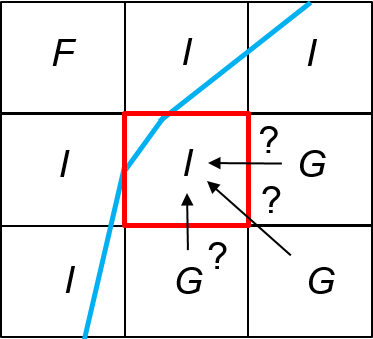
\includegraphics{figs/ps}
\caption{Example of a scenario in which particle distributions are missing post-streaming.}
\label{fig:ps}
\end{figure}

The missing particle distributions need to be reconstructed.
Also, momentum needs to be conserved at the interface.
When the particle distributions are reconstructed, they will be reconstructed in such a way that momentum is conserved between the primary fluid and the secondary fluid.
In order to perform the reconstruction, there are a few assumptions that need to be made:
\begin{enumerate}
\item The velocity of the secondary fluid is equal to the velocity of the primary fluid at the free-surface, i.e. there is no-slip between the two-fluids.
\item The secondary fluid is at equilibrium and at constant pressure, $p_G$.
\item There is a force balance for opposite lattice directions.
\end{enumerate}
Because particle distributions are a measure of momentum transport, the pressure of the secondary fluid can be converted to the particle distribution scale and the missing particle distribution can be solved for algebraically.
Consider \Fref{fig:fbi}.
Balancing the opposite lattice directions results in:
\begin{eqnarray}
f_i + f_\opidx &=& f^{eq}_\opidx(\rho_G, \mathbf{u}) + f_i^{eq}(\rho_G, \mathbf{u}), \\
\label{eq:reconst} f_\opidx &=& f_\opidx^{eq}(\rho_G, \mathbf{u}) + f_i^{eq}(\rho_G, \mathbf{u}) - f_i.
\end{eqnarray}
Missing distribution functions can be reconstructed according to \eqref{eq:reconst}.
In order for conservation of momentum to be satisfied along the free-surface, distribution functions coming from the direction of the interface normal, $\mathbf{n}$, must also be reconstructed.
Thus, distribution functions are reconstructed if coming from a gas cell, or if $\mathbf{n} \cdot \pvel_\opidx > 0$.

\begin{figure}
\centering
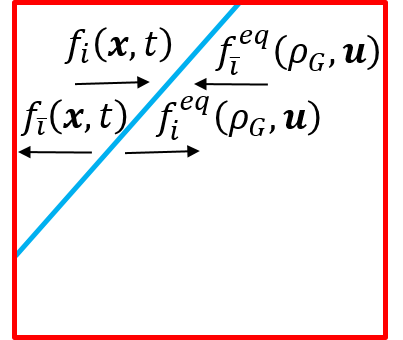
\includegraphics{figs/force-bal-at-interface}
\caption{Particle distributions at free-surface for a pair of opposing lattice directions after gas pressure, $\rho_G$, is in the particle distribution form.}
\label{fig:fbi}
\end{figure}

\subsection{Resulting Algorithm for Simulating Free-Surface Flow using the Lattice Boltzmann Method}

For clarity, the complete algorithm used in the current work for simulating free-surface flow using the Lattice Boltzmann Method is presented in \Fref{algo:free-surface-complete}.

\begin{algorithm}
\caption{Free-Surface Flow using the Lattice Boltzmann Method} \label{algo:free-surface-complete}
\begin{algorithmic}[1]
  \Procedure{FreeSurfaceLBM}{$\rho_0$, $u_0$, $M_0$, $t_{max}$} \Comment{$\rho_0$, $u_0$, $M_0$ specify initial conditions}
\Statex \Comment{Initialize data structures}
\State Initialize $\rho(\pos, 0)$ and $\mathbf{u}(\pos, 0)$ to initial conditions
%\Statex \Comment{Quasiequilibrium is defined in \Fref{eq:
\State Initialize $f$ to quasiequilibrium, $f_i(\pos, 0) = f_i^{eq}(\rho(\pos, 0), \mathbf{u}(\pos, 0))$

\Statex \Comment{Main loop}
\For{$t = 0:\Delta t:t_{max}$}
\State Mass transfer, $M(\pos, t + \Delta t) = M(\pos, t) + \sum_i \Delta M_i(\pos, t)$, (\Fref{sec:mass-transfer})
  \Statex \Comment{$\pvel_i$ depends on lattice}
  \State Stream particle distributions, $f_i(\pos + \pvel_i \Delta t, t + \Delta t) = f_i(\pos, t)$ 
  \State Reconstruct particle distributions (\Fref{sec:bc-at-fs})
  \State Particle collisions (\Fref{sec:colop})
  \State Enforce boundary conditions (\Fref{sec:bcs})
  \State Calculate macroscopic variables
  \State Update cell states (\Fref{algo:update-cell-updates})
\EndFor
\Statex
\State Post-process
\EndProcedure
\end{algorithmic}
\end{algorithm}


\newcommand{\nodesi}{50}
\newcommand{\nodesj}{500}
\newcommand{\anw}{$1\frac{1}{4}$"}
\newcommand{\anh}{1'}
\newcommand{\nsteps}{16000}

\section{Numerical Study of Primary Cementing} \label{sec:results}

The free-surface LBM model was implemented and used to simulate primary cementing in a dry annulus, i.e. an annulus without drilling mud.
The focus of the current study was the performance of different characteristic flow behaviors (as could potentially relate to different cement slurry mixes) when used to cement different imperfect wellbore geometries.
Because the focus in regards to the wellbore is on geometrical imperfections, the entire wellbore annulus is not simulated, but instead a small section around a geometrical imperfection is considered.
A schematic of an example primary cementing simulation, including boundary conditions, is shown in \Fref{fig:wellbore-cementing-schematic}.

\begin{figure}
\centering
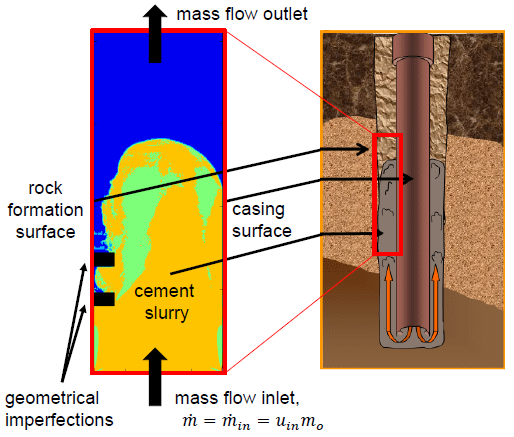
\includegraphics{figs/wellbore-cementing-schematic}
\caption{Example simulation used in primary cementing study.
The black rectangles on the left boundary represent notches protruding from the rock formation surface. The contours are of the primary fluid (cement slurry) mass.
The schematic on the right is courtesy of~\cite{cementing2015web}}.
\label{fig:wellbore-cementing-schematic}
\end{figure}

%The simulations were carried out on a $\nodesi \times \nodesj$ lattice, which corresponds to an annulus width of \anw \hspace{0.05cm} and a sectional height of \anh.
The simulations were carried out on a $\nodesi \times \nodesj$ lattice.
For the mass inlet, a~\citet{zou1997pressure} velocity boundary condition was used in conjuction with a constant mass boundary condition, i.e. $M(\pos_j, t) = M_0 = 1.0$ for all $\pos_j$ along the inlet.
This corresponded to a constant mass flow, $\dot{M}_{in} = M_0 u_0$, at inlet.
For the outlet, mass was allowed to transfer out of the domain during the mass transfer step such that $f_\opidx(\pos + \pvel_i \Delta t, t) = 0$ in \eqref{eq:dM} for all $\pos + \pvel_i \Delta t$ that lie outside of the domain on the other side of the mass outlet (i.e. the boundary condition at the outlet is such that there is no backflow).
All simulations were executed for $\nsteps$ time steps.

The different imperfect geometries that were considered at the rock formation surface were: flow over a cavity that is 30\% of the annulus width, ``cav $30 \times 1$''; flow over a cavity that is 60\% of the annulus width, ``cav $60 \times 1$''; flow over a square obstacle with sides that are 30\% of the annulus width, ``obs $30 \times 1$''; flow over two square obstacles with sides that are 30\% of the annulus width, ``obs $30 \times 2$''; flow over a square obstacle with sides that are 60\% of the annulus width, ``obs $60 \times 1$''; flow over two square obstacles with sides that are 60\% of the annulus width, ``obs $60 \times 2$''; and flow over a rectangular obstacle with width that is 60\% of the annulus width and length that is four times the width, ``obs $60 \times L$''.
The wellbore geometries that were considered herein are depicted in \Fref{fig:wellbore-geometries}.

\begin{figure}
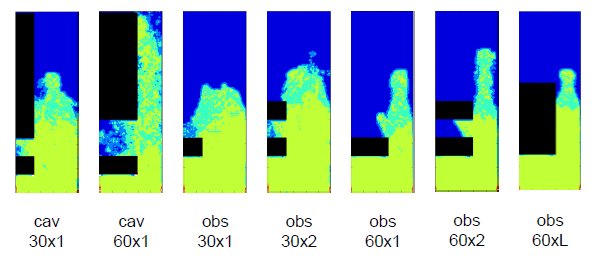
\includegraphics[width=\linewidth]{figs/wellbore-geometries}
\caption{Wellbore geometries considered in the study.}
\label{fig:wellbore-geometries}
\end{figure}

In addition to wellbore geometry, different cement slurry material properties and cement slurry flow rates were considered, which are characterized by the dimensionless Reynold's number, $Re = \frac{\rho U L}{\mu_p}$, and Bingham number, $Bn = \frac{\tau_y L}{\mu_p U}$, of the flow, where $L \equiv $ the width of the annulus.
A particular goal of the study was to investigate which Reynold's numbers and Bingham numbers were preferable for each geometry, and which Reynold's numbers and Bingham numbers performed well for all geometries.
The dimensionless numbers were defined as follows, $(Re, Bn) = (1.00, 4.00)$,  $(2.50, 0.00)$, $(2.50, 1.00)$, $(2.50, 10.0)$, $(2.50, 25.0)$, $(5.00, 5.00)$, and $(12.5, 2.0)$.
\Fref{fig:percent-filled} shows the percentage of the wellbore annulus section filled at the end of the cement simulation duration.
The percent fill was calculated as:
\begin{equation}
  \frac{\sum\limits_{\pos \in \domain} \epsilon(\pos, 16000)}{\sum\limits_{\pos \in \domain} 1.0}.
\end{equation}

\begin{figure}
\centering
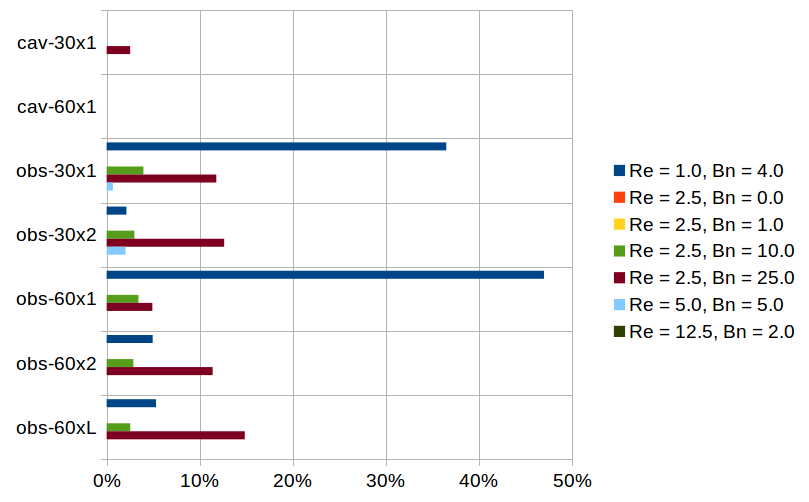
\includegraphics[width=\linewidth]{figs/percent_filled}
\caption{Percent of voids in wellbore at the end of simulation for each cement slurry flow through each wellbore geometry.}
\label{fig:percent-filled}
\end{figure}

Based upon \Fref{fig:percent-filled}, some general statements can be made about what properties of the cement slurry flow are preferable.
For example, low yield stress, and consquently low Bingham number flows ($Bn \le 1.0$), approximately completely filled the annulus for every wellbore geometry considered.
In addition, the negligible percentage of voids for the ($Re = 5.00, Bn = 5.00$) and ($Re = 12.5, Bn = 2.0$) slurry flows suggests that if the ratio of $Bn / Re$ is low, that the slurry flow will result in a low percentage of voids for cementing a dry hole as is desired.
As $Bn / Re$ increases, it appears that, in certain cases and wellbore geometries, the slurry flow tends to result in a larger percentage of voids (approximately 10\%-40\%). \pagebreak
What is interesting to note is that for slurry flows that resulted in a percentage of voids greater than 3\%, there was a lack of consistency across wellbore geometries in terms of which slurry flow resulted in more voids and which slurry flow resulted in less, which suggests that generalities cannot always be made and that computational methods are necessary for understanding and designing slurry mixes for real-life wellbores.

\section{Conclusions} \label{sec:conclusion}

An LBM model for simulating non-Newtonian and free-surface flow to represent cementing dry annuli in oil and gas wellbores was presented.
The model was then used to study how different cement slurry flows, defined by different Reynold's numbers and Bingham numbers, would perform in different wellbore geometries.
The results showed that in general, it is preferable that the yield stress and $Bn / Re$ ratio of the slurry flow be low.
However, beyond these considerations, it is not clear what slurry flow may be preferable for a given rock formation geometry.
The results suggest that computational methods are necessary for (a) better understanding the mechanics of primary cementing and (b) for designing a cement mix for a given wellbore.
The lattice Boltzmann method extended for simulating non-Newtonian and free-surface flow as presented in the current work has several properties that make it a good candidate for such a design framework:
\begin{itemize}
\item LBM is well-suited for simulating non-Newtonian fluids because the strain-rate tensor is computed local to each node and is second-order accurate~\cite{kruger2009shear,kruger2010second}.
\item LBM is well-suited for simulating multiphase multicomponent flow and free-surface flow because it can handle complicated interface shapes between fluid phases and components.
\item LBM is easily written in parallel and as hardware architectures shifts sequential to parallel computing, it becomes increasingly important that code for simulating complex and computationally expensive phenomena be written in parallel.
\item The LBM no-slip boundary condition works well with complex geometries, such as those that occur in realistic rock formation surfaces in drilled wellbores.
\end{itemize}

Future work would include developing a more physically realistic model.
Primary cementing can involve multiple phases and multiple components, namely the cement slurry, a spacer fluid, and drilling mud.
Possible future work would be to make the model more general so as to be capable of simulating multiphase multicomponent flow.
In addition, a more physically realistic model would simulate three-dimensional flow so as to be able to simulate eccentric annuli and three-dimensional rock formation imperfections.


